\documentclass[11pt]{article}
\usepackage[margin=1in]{geometry}
\usepackage{graphicx}
\usepackage{amsmath, amssymb}
\usepackage{booktabs}
\usepackage{listings}
\usepackage{xcolor}
\usepackage{hyperref}
\usepackage{caption}
\usepackage{subcaption}

\definecolor{codebg}{RGB}{245,245,250}
\lstset{basicstyle=\ttfamily\small, backgroundcolor=\color{codebg},
        breaklines=true, frame=single, framesep=4pt,
        showstringspaces=false}

\hypersetup{colorlinks=true, urlcolor=blue, linkcolor=black}

\title{A Three-Loop Magnetic-Field Array for Polarization-Independent
HF Reception\\\large Geometry, Direction-Dependent Projection,
Polarimetry, and a Validation Pipeline}
\author{}
\date{\today}

\begin{document}
\maketitle

\begin{abstract}
We describe a compact three-element magnetic-loop antenna array in which
the loops sit on three faces of a cube whose body diagonal is vertical
and whose lower vertex rests on the ground.  This geometry makes the
three loop normals identically tilted from the zenith and uniformly
spaced in azimuth.  We derive the linear transformation that takes the
three measured magnetic-field components to the lab-frame magnetic
field, and from there to the wave's magnetic field projected onto a
plane perpendicular to a chosen arrival direction.  The resulting
$|\mathbf{B}_\perp|^2$ is a polarization-independent intensity estimator;
the same projection plus a complex-baseband extraction yields the
Stokes parameters and hence the polarization state of the wave.  A
companion Python module implements the full pipeline and is validated
on a simulated 20\,MHz signal with controllable Faraday rotation and
additive noise.
\end{abstract}

%-----------------------------------------------------------------------
\section{Coordinate systems and array geometry}
%-----------------------------------------------------------------------

We work in a right-handed lab frame with axes $(E, N, \mathrm{Up})$:
East, North, and the local vertical pointing up.  The arrival direction
of a plane wave is parameterized by an azimuth $\varphi$, measured
clockwise from North (so $\varphi = 0^\circ$ is N, $\varphi = 90^\circ$
is E), and an elevation $\theta$ measured upward from the local
horizontal.  The unit vector pointing \emph{toward the source} is
\begin{equation}
\hat{\mathbf{k}}(\varphi, \theta)
   = \bigl( \cos\theta\,\sin\varphi,\;
            \cos\theta\,\cos\varphi,\;
            \sin\theta \bigr)^{\!\top}.
\label{eq:khat}
\end{equation}
Figure~\ref{fig:azel} shows the convention.

\begin{figure}[h]
\centering
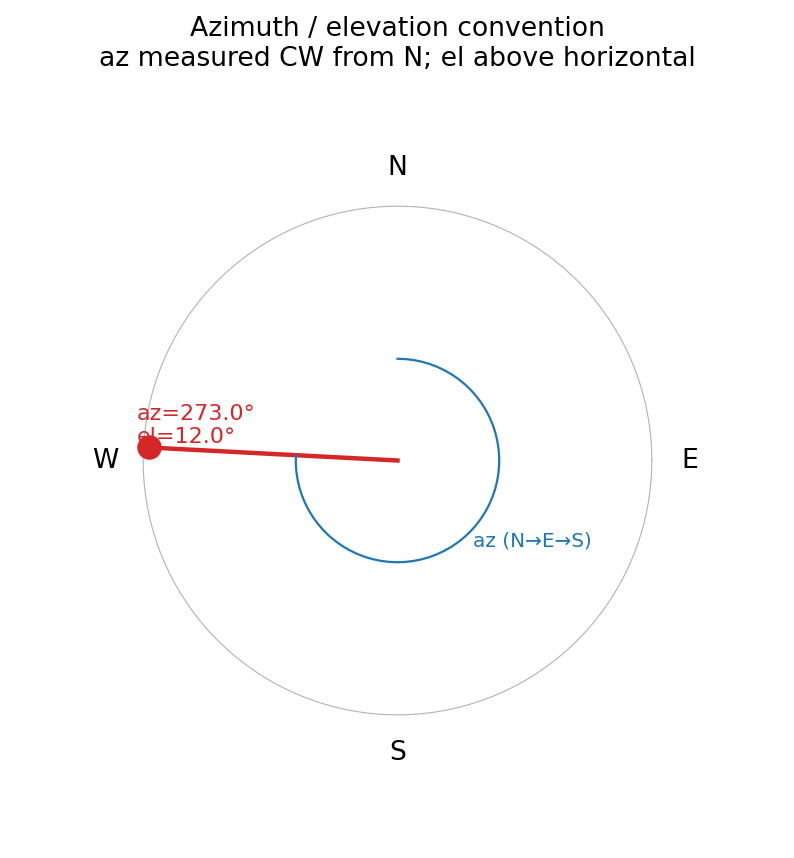
\includegraphics[width=0.55\linewidth]{figures/az_el_convention.png}
\caption{Azimuth/elevation convention.  $\varphi$ is measured clockwise
from N (so the sequence is $\mathrm{N}\!\to\!\mathrm{E}\!\to\!\mathrm{S}
\!\to\!\mathrm{W}$); $\theta$ is the elevation above the horizontal.
The red dot illustrates a wave arriving from $\varphi = 273^\circ$,
$\theta = 12^\circ$, the approximate path of WWV $\to$ Cambridge MA.}
\label{fig:azel}
\end{figure}

\subsection*{Cube on a vertex}

Consider a unit cube standing on its $(0,0,0)$ corner with its body
diagonal aligned to the lab-frame vertical.  The three faces meeting at
that lower vertex have outward normals each tilted
\(\arccos(1/\sqrt{3}) = 54.7356^\circ\) from the zenith
(equivalently, $35.26^\circ$ above the horizontal), and their horizontal
projections are spaced $120^\circ$ apart in azimuth.  The three loops
are placed flat on those faces, so the $i$-th loop senses the magnetic-field
component along the corresponding face normal $\hat{\mathbf{n}}_i$.

We label the loops L1, L2, L3 with horizontal-projection azimuths of
$0^\circ$, $+120^\circ$, $-120^\circ$ respectively.  Loop L1's normal
points ``N + up''; L2's points roughly ``S-of-east + up''; L3's points
roughly ``S-of-west + up''.  In lab coordinates,
\begin{equation}
\boxed{\;
\mathsf{N} \;=\;
\begin{pmatrix}
\hat{\mathbf{n}}_1^{\!\top} \\[2pt]
\hat{\mathbf{n}}_2^{\!\top} \\[2pt]
\hat{\mathbf{n}}_3^{\!\top}
\end{pmatrix}
\;=\;
\begin{pmatrix}
0                       & \sqrt{2/3}    & \tfrac{1}{\sqrt{3}}\\[3pt]
+\sin 54.74^\circ\sin 120^\circ &
\sin 54.74^\circ\cos 120^\circ & \tfrac{1}{\sqrt{3}}\\[3pt]
-\sin 54.74^\circ\sin 120^\circ &
\sin 54.74^\circ\cos 120^\circ & \tfrac{1}{\sqrt{3}}
\end{pmatrix}.
}
\label{eq:N}
\end{equation}
Figures~\ref{fig:cube} and~\ref{fig:topdown} illustrate the geometry.

\begin{figure}[h]
\centering
\begin{subfigure}[t]{0.49\linewidth}\centering
  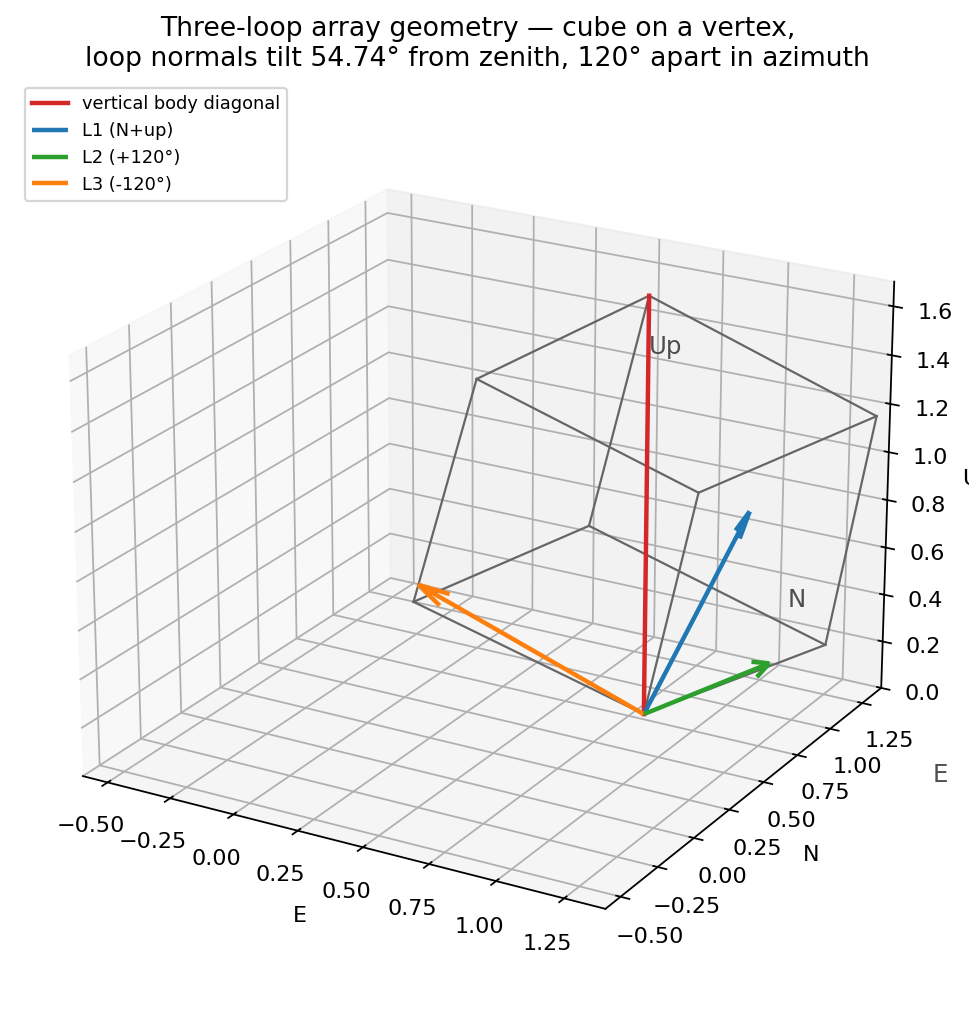
\includegraphics[width=\linewidth]{figures/geometry_cube.png}
  \caption{3-D view: cube on a vertex with the body diagonal vertical
  (red).  The blue/green/orange arrows are the three loop normals
  $\hat{\mathbf n}_1, \hat{\mathbf n}_2, \hat{\mathbf n}_3$.}
  \label{fig:cube}
\end{subfigure}\hfill
\begin{subfigure}[t]{0.49\linewidth}\centering
  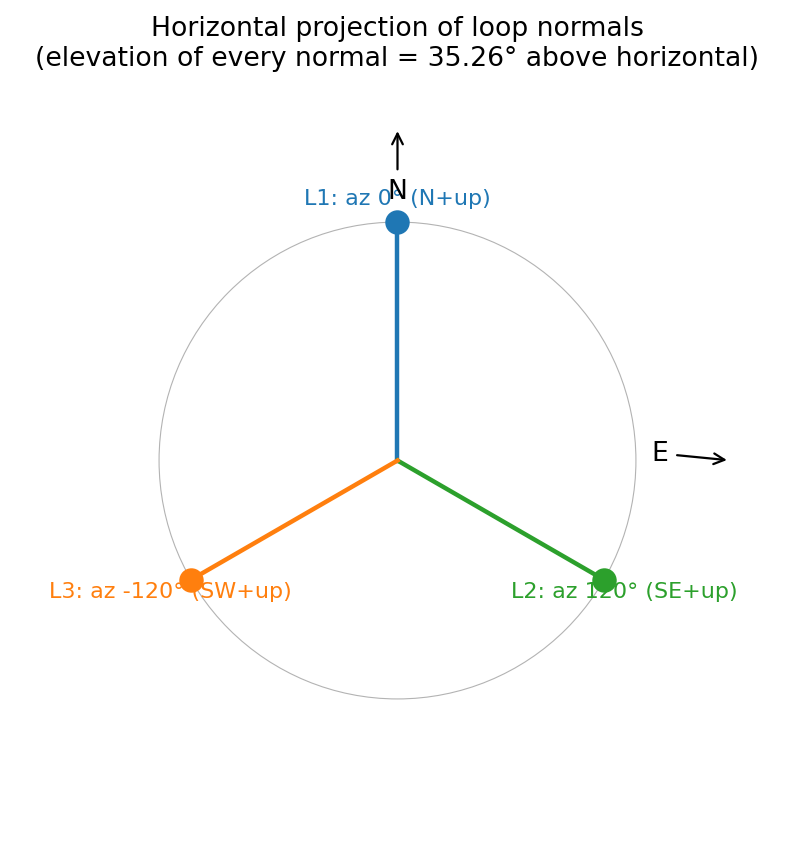
\includegraphics[width=\linewidth]{figures/normals_top_down.png}
  \caption{Top-down: the horizontal projections of the three normals
  are $120^\circ$ apart.  All three normals tilt $35.26^\circ$ above
  the horizontal.}
  \label{fig:topdown}
\end{subfigure}
\caption{Geometry of the cube-vertex three-loop array.}
\end{figure}

\subsection*{From three measurements to the lab-frame B vector}

Each loop senses
$B_i(t) = \hat{\mathbf{n}}_i \cdot \mathbf{B}_{\mathrm{lab}}(t)$, so
\begin{equation}
\begin{pmatrix} B_1(t)\\ B_2(t)\\ B_3(t) \end{pmatrix}
\;=\; \mathsf{N}\,\mathbf{B}_{\mathrm{lab}}(t),
\qquad
\mathbf{B}_{\mathrm{lab}}(t) \;=\; \mathsf{N}^{-1}
\begin{pmatrix} B_1(t)\\ B_2(t)\\ B_3(t) \end{pmatrix}.
\label{eq:Ninv}
\end{equation}
The three rows of $\mathsf{N}$ have unit length but are not mutually
orthogonal --- their pairwise inner product is $1/3$ (an artefact of
the cube geometry).  Hence one must take the proper inverse,
not the transpose.  $\mathsf{N}$ depends only on the array geometry,
not on frequency; per-loop frequency response is a separate scalar
calibration that should be folded into the $B_i$'s before \eqref{eq:Ninv}
is applied.

%-----------------------------------------------------------------------
\section{Direction-dependent projection}
%-----------------------------------------------------------------------

A plane electromagnetic wave has $\mathbf{B}\perp\hat{\mathbf k}$ at all
times, so to obtain a polarization-independent estimator of intensity
arriving from direction $\hat{\mathbf k}$ we project the lab-frame
$\mathbf B$ onto the plane perpendicular to $\hat{\mathbf k}$:
\begin{equation}
\mathbf{B}_{\!\perp}(t)
   = \bigl(\mathsf{I} - \hat{\mathbf k}\hat{\mathbf k}^{\!\top}\bigr)
     \mathbf{B}_{\mathrm{lab}}(t)
   = \mathsf{P}(\hat{\mathbf k})\,\mathsf{N}^{-1}
     \begin{pmatrix} B_1(t)\\ B_2(t)\\ B_3(t) \end{pmatrix}.
\label{eq:Bperp}
\end{equation}
The polarization-independent intensity is then
\begin{equation}
P(\varphi,\theta;t) \;=\; |\mathbf{B}_\perp(t)|^2
   \;=\; \bigl(B_1\;B_2\;B_3\bigr)\,\mathsf{M}^{\!\top}\mathsf{M}\,
         \begin{pmatrix} B_1\\ B_2\\ B_3\end{pmatrix},
\quad\text{with}\quad
\mathsf{M} \equiv \mathsf{P}(\hat{\mathbf k})\,\mathsf{N}^{-1}.
\label{eq:intensity}
\end{equation}
Time-averaging $|\mathbf B_\perp|^2$ recovers a beamformed power for
the chosen $\hat{\mathbf k}$.  The instantaneous form preserves the
amplitude trace of the polarization-independent envelope.

\paragraph{Sign flip across a loop plane.}
When the source elevation passes through the plane containing one of
the loops, the projection coefficient $\hat{\mathbf n}_i\!\cdot\!\hat{\mathbf k}$
goes through zero and reverses sign.  Because that coefficient enters
the projector multiplicatively, the math handles the sign change
naturally, but the corresponding loop's contribution to the
\emph{phase} of $\mathbf B_\perp$ flips by $180^\circ$ at the crossing.
Phase tracking through such transitions therefore requires either
selecting a $\hat{\mathbf k}$ that avoids them or carrying the sign
explicitly.  The intensity estimator is unaffected because it is
quadratic.

%-----------------------------------------------------------------------
\section{Polarimetry: the Stokes parameters}
%-----------------------------------------------------------------------

Construct two unit vectors $\hat{\mathbf p}, \hat{\mathbf q}$ that span
the plane perpendicular to $\hat{\mathbf k}$ (Figure~\ref{fig:perpbasis}).
A natural choice is
\begin{equation}
\hat{\mathbf p} \;=\; \frac{\hat{\mathbf k}\times\hat{\mathbf z}_{\mathrm{Up}}}
                            {|\hat{\mathbf k}\times\hat{\mathbf z}_{\mathrm{Up}}|},
\qquad
\hat{\mathbf q} \;=\; \hat{\mathbf k}\times\hat{\mathbf p},
\end{equation}
so that $\hat{\mathbf p}$ lies in the local horizontal plane and
$\hat{\mathbf q}$ is generally upward.  After narrow-band complex
baseband extraction (Section~\ref{sec:pipeline}) we obtain three
complex time-series $z_i(t)$ for the loops, which we map to the lab
frame
$\mathbf{Z}_{\mathrm{lab}} = \mathsf{N}^{-1}\,\mathbf{z}$,
project onto the plane perpendicular to $\hat{\mathbf k}$,
$\mathbf{Z}_{\!\perp} = \mathsf{P}\,\mathbf{Z}_{\mathrm{lab}}$,
and decompose into the two complex polarization components
\begin{equation}
A_p(t) \;=\; \hat{\mathbf p}\cdot\mathbf{Z}_{\!\perp}(t),
\qquad
A_q(t) \;=\; \hat{\mathbf q}\cdot\mathbf{Z}_{\!\perp}(t).
\end{equation}

\begin{figure}[h]\centering
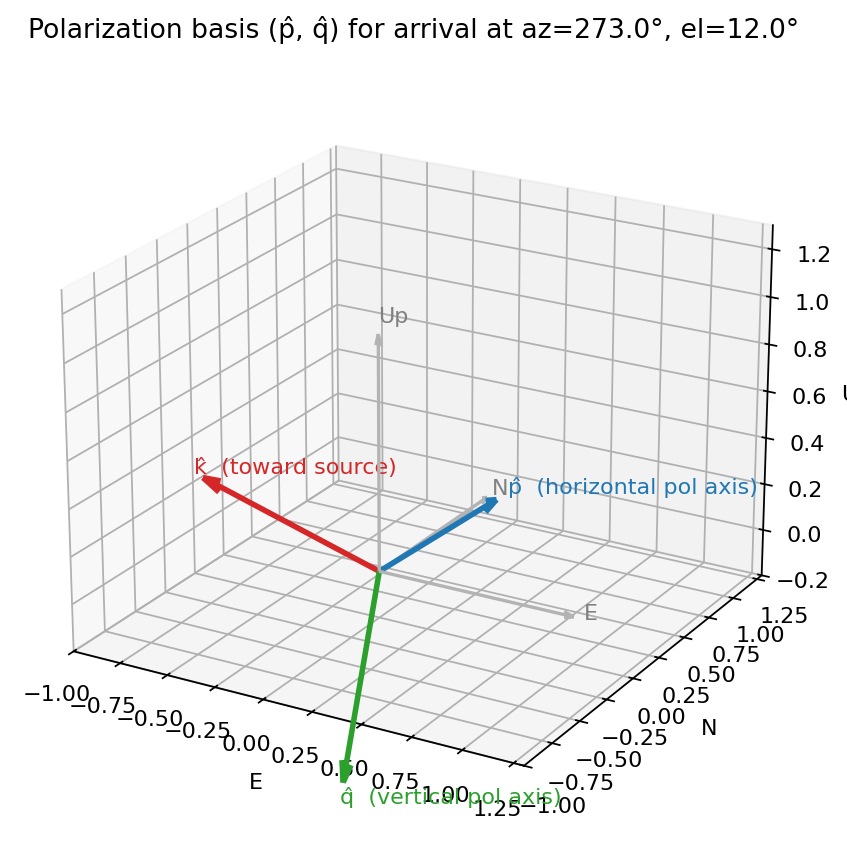
\includegraphics[width=0.5\linewidth]{figures/perp_basis.png}
\caption{Polarization basis at the example arrival direction
$\varphi = 273^\circ$, $\theta = 12^\circ$.  $\hat{\mathbf p}$ lies in
the local horizontal plane; $\hat{\mathbf q}$ is the orthogonal
direction in the wave plane.}
\label{fig:perpbasis}
\end{figure}

The Stokes parameters are the standard quadratic combinations:
\begin{equation}
\begin{aligned}
I &= |A_p|^2 + |A_q|^2,\\
Q &= |A_p|^2 - |A_q|^2,\\
U &= 2\,\Re\!\bigl[A_p^*\,A_q\bigr],\\
V &= 2\,\Im\!\bigl[A_p^*\,A_q\bigr].
\end{aligned}
\label{eq:stokes}
\end{equation}
The polarization fraction is $\Pi = \sqrt{Q^2+U^2+V^2}/I$,
the position angle of the linear part is
$\chi = \tfrac{1}{2}\arctan(U,Q)$, and the ellipticity is
$\eta = \tfrac{1}{2}\arctan\!\bigl(V/\sqrt{Q^2+U^2}\bigr)$
(linear if $\eta=0$, RCP if $\eta=+45^\circ$, LCP if $\eta=-45^\circ$).

%-----------------------------------------------------------------------
\section{Implementation: pipeline and code}
\label{sec:pipeline}
%-----------------------------------------------------------------------

The accompanying Python module \texttt{three\_loop.py} implements the
pipeline:
\begin{enumerate}\itemsep=2pt
\item Read $(t, B_1, B_2, B_3)$ for the three loops.
\item For each loop, find the spectral peak nearest a user-supplied
      target carrier $f_0$ within a search window $\pm BW/2$.
\item Mix to baseband at the detected peak frequency and apply a
      brick-wall low-pass filter at $\pm BW/2$ to obtain narrow-band
      complex signals $z_i(t)$.
\item Form $\mathbf{Z}_{\mathrm{lab}} = \mathsf{N}^{-1}\mathbf{z}$,
      $\mathbf{Z}_{\!\perp} = \mathsf{P}(\hat{\mathbf k})\,
      \mathbf{Z}_{\mathrm{lab}}$.
\item Compute the polarization-independent intensity
      $|\mathbf{Z}_{\!\perp}(t)|^2$.
\item Decompose onto $(\hat{\mathbf p},\hat{\mathbf q})$, compute Stokes,
      polarization fraction, ellipticity, position angle.
\item Estimate the dominant polarization eigenvector and return the
      instantaneous amplitude, phase, and frequency on that channel.
\end{enumerate}

\noindent The signature is
\begin{lstlisting}[language=Python]
from three_loop import analyze
out = analyze(t, B1, B2, B3,
              f0,        # target carrier (Hz)
              BW,        # search/extract bandwidth (Hz)
              az_deg,    # initial guess azimuth, deg from N CW
              el_deg)    # initial guess elevation, deg above horizon
# out: amp_dominant, instant_phase, instant_freq, intensity,
#      stokes (I,Q,U,V), pol_fraction, ellipticity_deg,
#      position_angle_deg, ...
\end{lstlisting}

%-----------------------------------------------------------------------
\section{Validation: simulated WWV at 20\,MHz from Fort Collins}
%-----------------------------------------------------------------------

The simulator \texttt{simulate\_wwv()} synthesizes a known plane wave
arriving from a chosen direction with a chosen polarization, optionally
including a constant or rotating Faraday angle and additive Gaussian
noise.  We use it to validate the analysis pipeline.

The great-circle bearing from Fort Collins, CO ($40.59^\circ$\,N,
$105.08^\circ$\,W) to Cambridge, MA ($42.37^\circ$\,N, $71.11^\circ$\,W)
is $273^\circ$ (slightly N of due west).  For a single-hop F-region
sky-wave reflecting at $\sim 300$\,km altitude over a $\sim 2840$\,km
great-circle distance, the takeoff/arrival elevation is
$\theta = \arctan(300/(2840/2)) \approx 12^\circ$.  We therefore inject
a wave with $\varphi = 273^\circ$, $\theta = 12^\circ$, an IF
representation of the 20\,MHz carrier, and various polarization
states.

\begin{figure}[h]\centering
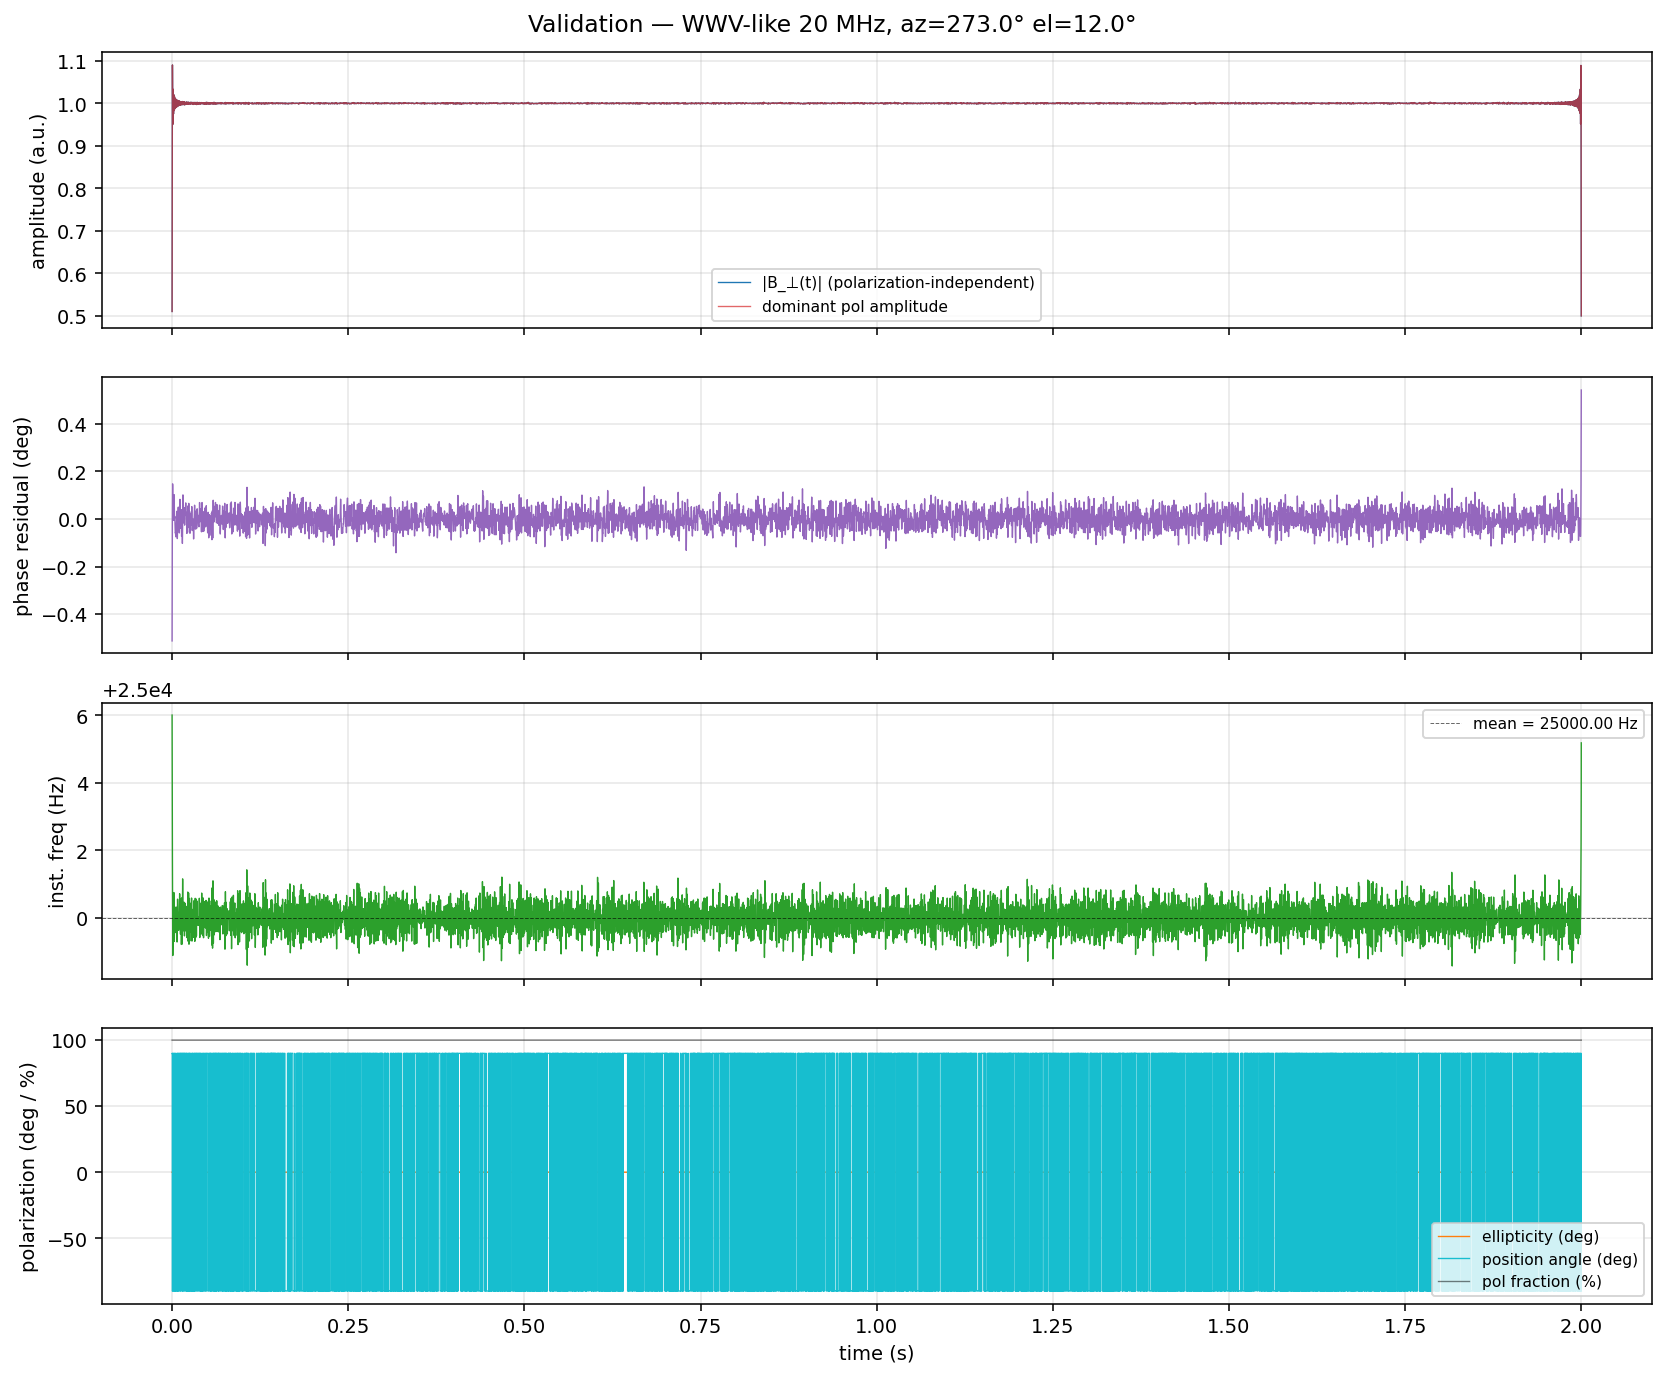
\includegraphics[width=0.95\linewidth]{figures/validation_20MHz.png}
\caption{Validation run: linear-vertical polarization injected at
$\varphi=273^\circ$, $\theta=12^\circ$, recovered with no Faraday
rotation, SNR $= 40$\,dB per channel.  The recovered carrier frequency
matches the truth to better than a millihertz over the 2-second
recording; the polarization fraction is $1.000$, the ellipticity is
$0^\circ$ (linear, as injected), and the position angle is $-89.9^\circ$
relative to $\hat{\mathbf p}$, i.e. along $-\hat{\mathbf q}$ which is
``vertical'' in the perpendicular plane.}
\end{figure}

\begin{figure}[h]\centering
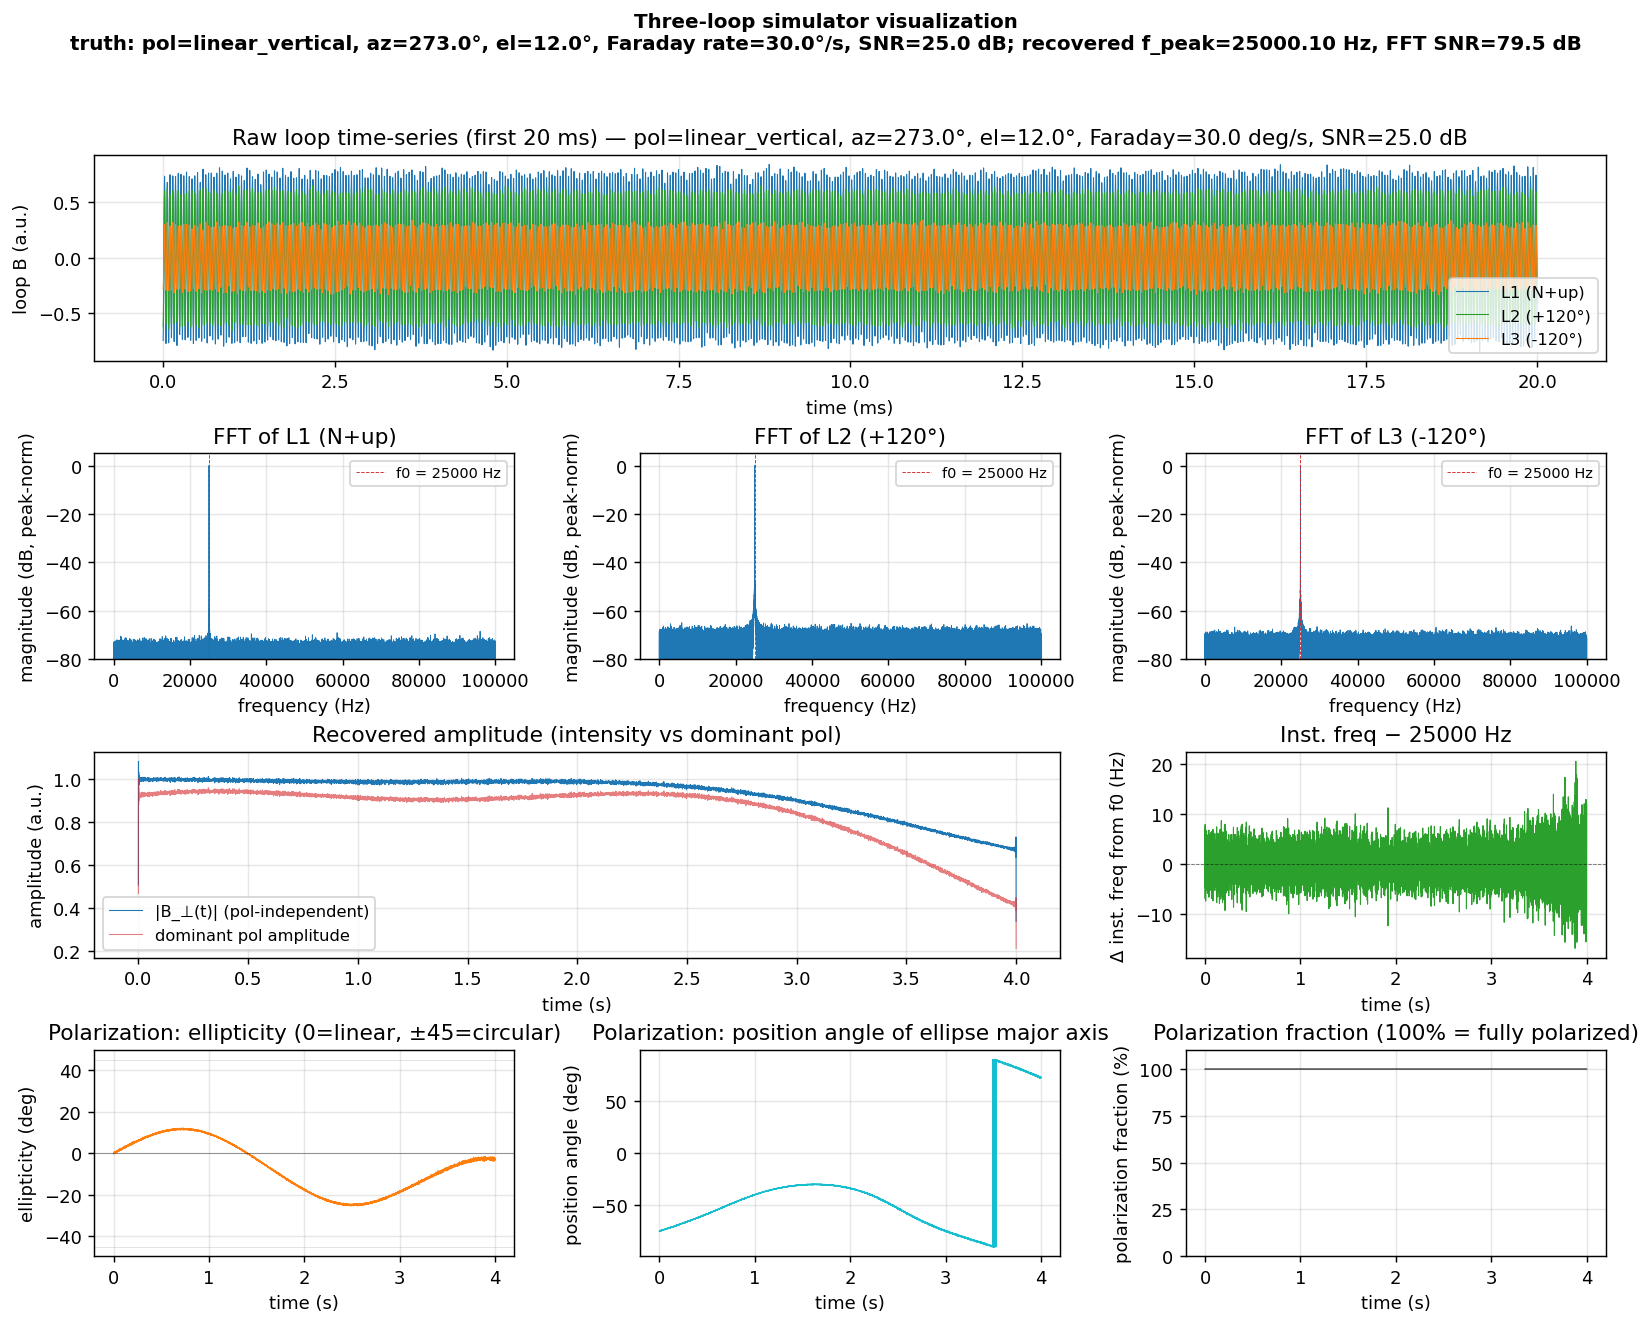
\includegraphics[width=0.95\linewidth]{figures/sim_linear_vertical_far30_snr25.png}
\caption{Linear-vertical input with Faraday rotation at $30^\circ$/s
and per-channel SNR of 25\,dB.  Top: raw loop time-series (first 20\,ms).
Second row: per-loop FFT spectra; the $\sim 25$\,kHz IF tone is
clearly visible above the noise floor in all three loops.  Third row:
recovered amplitude (the polarization-independent intensity is constant
to within noise, while the dominant-pol amplitude shows the
characteristic Faraday $|\cos\Omega(t)|$ modulation).  Fourth row:
polarization observables --- ellipticity stays near $0^\circ$ (linear
throughout), the position angle sweeps $30^\circ$/s as designed, and
the polarization fraction stays near 100\,\%.}
\end{figure}

\begin{figure}[h]\centering
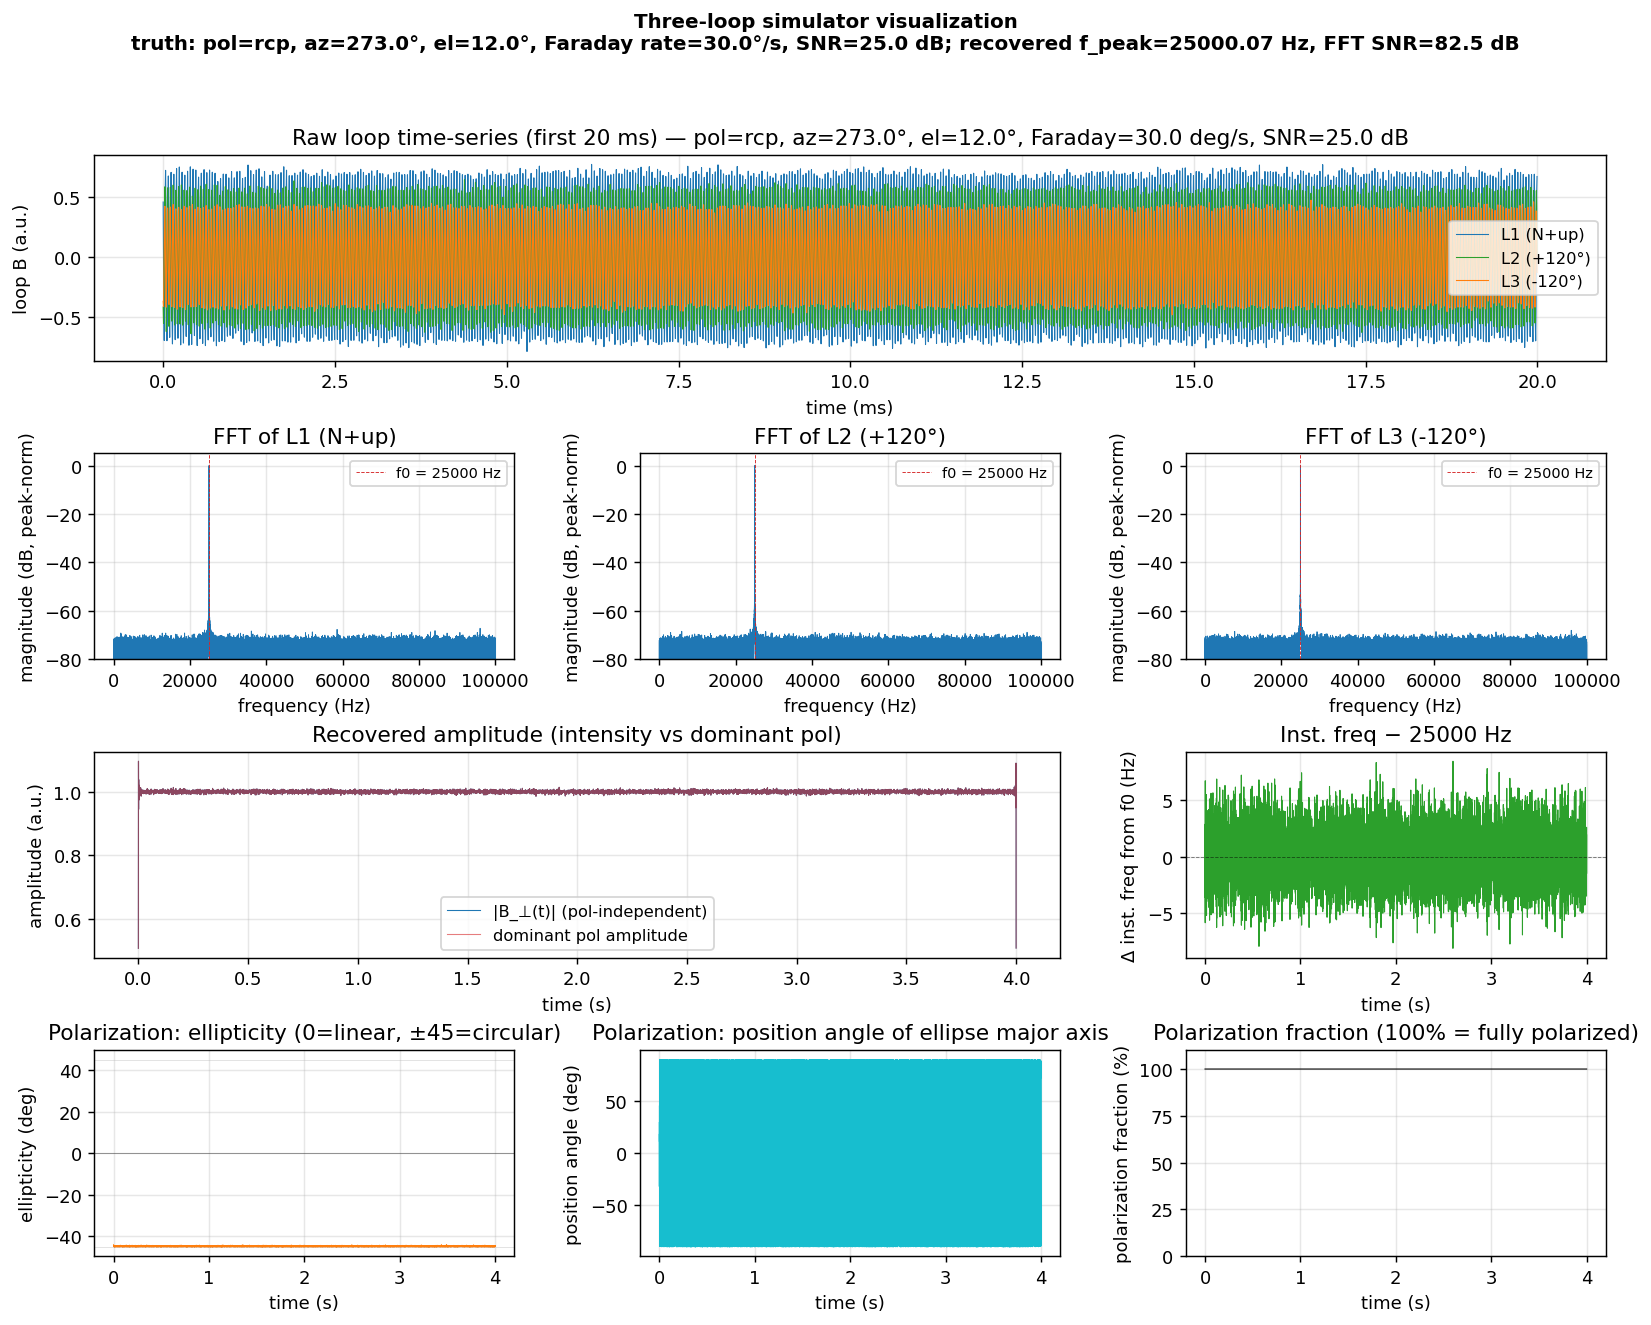
\includegraphics[width=0.95\linewidth]{figures/sim_rcp_far30_snr25.png}
\caption{RCP input with the same $30^\circ$/s Faraday rotation rate.
Now the polarization-independent intensity \emph{and} the dominant-pol
amplitude are constant (Faraday rotation just adds a common phase to
a circularly polarized wave), the ellipticity sits at $\pm 45^\circ$,
and the position-angle estimator becomes ill-defined as expected for
a circular wave.}
\end{figure}

%-----------------------------------------------------------------------
\section{Practical caveats}
%-----------------------------------------------------------------------

\begin{itemize}\itemsep=2pt
\item The geometry matrix $\mathsf{N}$ must be calibrated against the
      actual mechanical orientation of the loops --- a few-degree tilt
      error causes few-percent intensity miscalibrations and
      few-degree position-angle biases.

\item Each loop's effective area, gain, and phase response at the
      operating frequency must be matched.  In practice this is the
      dominant calibration burden; a known-direction CW beacon (or a
      stable HF transmission of known polarization) can be used to
      solve for per-channel complex gain corrections.

\item The single-point three-loop array has a $P(\hat{\mathbf k})
      = P(-\hat{\mathbf k})$ ambiguity: front and back are
      indistinguishable.  Resolving this requires either an additional
      E-field probe or a phased pair of three-loop triplets.

\item For unknown arrival direction, beamforming over a grid of
      $(\varphi,\theta)$ is suboptimal; the cleanest direction
      estimator is the eigendecomposition of the $3\times 3$
      covariance $\langle z_i\,z_j^*\rangle$, whose smallest-eigenvalue
      eigenvector is $\pm\hat{\mathbf k}$ (modulo the front/back
      ambiguity above).

\item All three loops must be sampled \emph{coherently} (shared LO and
      ADC clock).  An incoherent recording set --- e.g.\ three
      independent KiwiSDRs --- does not in general preserve the relative
      phase information needed for polarimetry.
\end{itemize}

\end{document}
